\documentclass[a4paper, 11pt, normalem]{report}

\usepackage{../../../LaTeX-Templates/Notes}
\usepackage{subfiles}

\title{Advanced Theoretical Physics \vspace{-20pt}}
\author{Dr Kendon and Prof Gardiner}
\date{\vspace{-15pt}Michaelmas Term 2019 - Epiphany Term 2020}
\rhead{\hyperlink{page.1}{Contents}}

\begin{document}

\maketitle
\tableofcontents

\part{Quantum Optics}
\chapter{}
\textbf{Syllabus:}
\begin{multicols}{2}
\begin{itemize}
    \item quantization of light
    \item creation and annihilation operators
    \item Hamiltonian of the E field
    \item number states
    \item coherent states
    \item squeezed states
    \item photon bunching and anti-bunching
    \item density operator
    \item pure states, mixed sates, entangled states
    \item decoherence
    \item atom-light interactions
    \item applications
\end{itemize}
\end{multicols}

\begin{figure}[H]
    \centering
    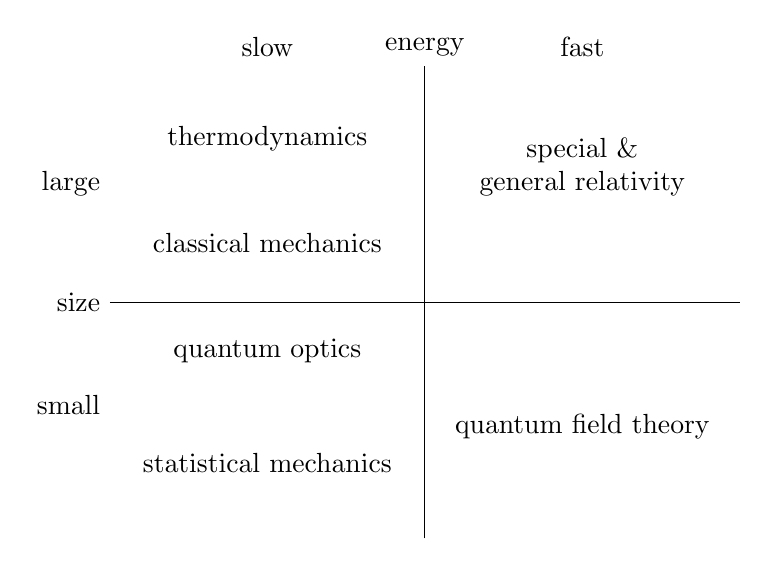
\begin{tikzpicture}
        \draw (-4,0) node[anchor=east] {size} -- (4,0);
        \draw (0,-3) -- (0,3) node[anchor=south] {energy};
        \draw[white] (-2.1,3) -- (-1.9,3) node[black,midway,anchor=south] {slow};
        \draw[white] (1.9,3) -- (2.1,3) node[black,midway,anchor=south] {fast};
        \draw[white] (-4,1.5) node[black,anchor=east] {large} -- (-3.9,1.5);
        \draw[white] (-4,-1.3) node[black,anchor=east] {small} -- (-3.9,-1.3);
        \draw[white] (-2.1,-0.35) -- (-1.9,-0.35) node[black,midway,anchor=north,align=center] {quantum optics};
        \draw[white] (-2.1,-1.8) -- (-1.9,-1.8) node[black,midway,anchor=north,align=center] {statistical mechanics};
        \draw[white] (-2.1,1.8) -- (-1.9,1.8) node[black,midway,anchor=south,align=center] {thermodynamics};
        \draw[white] (1.9,2.2) -- (2.1,2.2) node[black,midway,anchor=north,align=center] {\shortstack{special \&\\general relativity}};
        \draw[white] (1.9,-1.3) -- (2.1,-1.3) node[black,midway,anchor=north,align=center] {quantum field theory};
        \draw[white] (-2.1,0.5) -- (-1.9,0.5) node[black,midway,anchor=south,align=center] {classical mechanics};
    \end{tikzpicture}
\end{figure}

\textbf{Ingredients:}
\begin{itemize}
    \item harmonic oscillators
    \item Gaussian integrals
    \item Hamiltonian mechanics (canonical variables q and p)
    \item maths of operators - adjoint, self-adjoint, Hermitian, commutation relations
    \item QM in both Schrodinger and Heisenberg pictures
    \item density matrices
    \item classical EM - Maxwell's equations in Coulomb gauge - especially plane waves and dipoles
\end{itemize}

Hanbury Brown and Tiss:
\begin{equation}
    G(\tau) = I_A(t)I_B(t+\tau)
\end{equation}

\chapter{}
\section{Learning Outcomes}
To be able to state, explain and apply the operator formalism of the quantum harmonic oscillator, including:
\begin{itemize}
    \item the Hamiltonian in terms of the creation and annihilation operators
    \item the number operator and number states, eigenstates of the Hamiltonian
    \item definition of the creation and annihilation operators, commutation relations, adjoint and self-adjoint operators
    \item mathematical properties of the number states, completeness
    \item systems of two or more independent oscillators
\end{itemize}


\section{Quantum Harmonic Oscillator}
\begin{align}
    F &= ma = m\ddot{x} \\
      &= -kx \\
    x(t) &= x_0\sin\om t \\
    p_x(t) &= p_0\cos\om t \\
    V(x) &= \frac12 kx^2 = \frac12 m\om^2x^2 \\
    \frac{\hbar^2}{2m}\frac{d^2\psi}{dx^2} &+ V(x)\psi(x) = E\psi \\
    E_n &= \left(n+\frac12\right)\hbar\om
\end{align}
   
\begin{figure}[H]
    \centering
    \begin{tikzpicture}
        \draw[->,thick] (-3,0) -- (3,0) node[anchor=south] {$x$};
        \draw[->,thick] (0,-0.3) -- (0,2) node[anchor=south] {$V(x)$};
        \draw (0,0) parabola (2.5,1.8);
        \draw (0,0) parabola (-2.5,1.8);
    \end{tikzpicture}
\end{figure}
Start with writing the Hamiltonian, then turn everything into operators
\begin{align}
    H &= \frac{p^2}{2m} + \underbrace{\frac12 m\om^2x^2}_{V(x)} \\
    p &\to \hp = -i\hbar\frac{d}{dx},~ x \to \hx \\
    [\hx,\hp] &= i\hbar \\
    H &= \frac{\hp^2}{2m} + \frac12m\om^2\hx^2 \\
    \ha &= \frac{1}{\sqrt{2m\hbar\om}}\left(m\om\hx+i\hp\right) \\
    \hag &= \frac{1}{\sqrt{2m\hbar\om}} \left(m\om\hx - i\hp\right) \\
    \hx &= \left(\frac{\hbar}{2m\om}\right)^{1/2}(\ha+\hag) \\
    \hp &= -i\left(\frac{m\hbar\om}{2}\right)^{1/2}(\ha-\hag) \\
    [\ha,\hag] &= \ha\hag - \hag\ha = 1 \\
    \hh &= \hbar\om(\hag\ha+\frac12) \\
    \hag\ha &= \hn,~ \hn|n\rangle = n|n\rangle \\
    \hh|n\rangle &= \hbar\om\left(n+\frac12\right)|n\rangle = E_n|n\rangle
\end{align}
How do the annihilation and creation operators, $\ha$ and $\hag$ interact with the number states, $|n\rangle$?
\begin{align}
    \hag|n\rangle &= \sqrt{n+1}|n+1\rangle \\
    \ha|n\rangle &= \sqrt{n}|n-1\rangle
\end{align}
Together, the creation and annihilation operators are known as the \textit{ladder operators.}
Ladder operators move the system up or down the energy levels of the harmonic potential.
\begin{figure}[H]
    \centering
    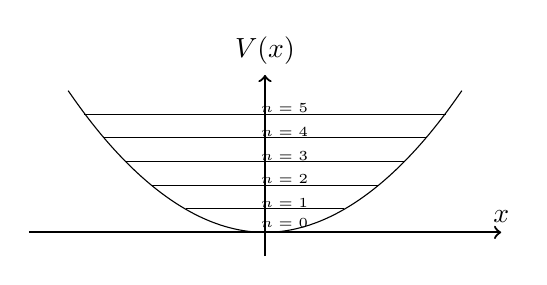
\begin{tikzpicture}
        \draw[->,thick] (-3,0) -- (3,0) node[anchor=south] {$x$} node[anchor=south,midway,xshift=7pt,yshift=-2pt] {\tiny $n=0$};
        \draw[->,thick] (0,-0.3) -- (0,2) node[anchor=south] {$V(x)$};
        \draw (0,0) parabola (2.5,1.8);
        \draw (0,0) parabola (-2.5,1.8);
        \draw (-2.3,1.5) -- (2.3,1.5) node[anchor=south,midway,xshift=7pt,yshift=-3pt] {\tiny $n=5$};
        \draw (-2.05,1.2) -- (2.05,1.2) node[anchor=south,midway,xshift=7pt,yshift=-3pt] {\tiny $n=4$};
        \draw (-1.78,0.9) -- (1.78,0.9) node[anchor=south,midway,xshift=7pt,yshift=-3pt] {\tiny $n=3$};
        \draw (-1.45,0.6) -- (1.45,0.6) node[anchor=south,midway,xshift=7pt,yshift=-3pt] {\tiny $n=2$};
        \draw (-1,0.3) -- (1,0.3) node[anchor=south,midway,xshift=7pt,yshift=-3pt] {\tiny $n=1$};
    \end{tikzpicture}
\end{figure}
We now have a partly new mathematical representation. 
Notice that the potential still remains positive, it does not go negative.
Therefore we must have:
\begin{align}
    \ha|0\rangle &= 0, \\
    \hn &= \hag\ha|0\rangle = 0. \\
    \implies \hh|0\rangle &= E_0|0\rangle = \frac12\hbar\om|0\rangle
\end{align}
So the ground state is labelled '0' but does not have $E=0$.\\
Now we introduce $\hog$ as the adjoint of $\ho$ if
\begin{align}
    \langle\psi|\ho|\phi\rangle &= \langle\phi|\hog|\psi\rangle^*\; \forall \psi,\phi
\end{align}
A self-adjoint operator is equivalent to a Hermitian operator, i.e. $\hn, \hh$.\\
For adjoint operators:
\begin{align}
    (\hat{A}+\hat{B})^\dagger &= \hat{A}^\dagger + \hat{B}^\dagger \\
    (\hat{A}\hat{B})^\dagger &= \hat{B}^\dagger\hat{A}^\dagger \\
    (c\hat{A})^\dagger &+ c^*\hat{A}^\dagger \\
    (\hat{A}^\dagger)^\dagger &= \hat{A}
\end{align}
More on the number states:
\begin{itemize}
    \item they are orthogonal
        \begin{align}
            \langle n|n\rangle &= 1 \\
            \langle n|m\rangle &= 0,~ n\neq m \\
            \langle n|m\rangle &= \delta_{n,m} \\
        \end{align}
    \item they form a basis (note: not mathematically a Hilbert space, but a Banah(?) space)
        \begin{align}
            |\psi\rangle &= \sum_n c_n|n\rangle \\
            0 &\leq n \leq \infty
        \end{align}
\end{itemize}

\section{Two Oscillators - independent}
\begin{align}
    |\psi_0\rangle &= \sum_n c_n|n\rangle_0 \\
    |\psi_1\rangle &= \sum_m c_m|m\rangle_1 \\
    |\psi_{01}\rangle &= \sum_{n,m} c_{n,m}|n\rangle_0|m\rangle_1
\end{align}
What we are doing is "tensoring" the Hilbert spaces: $\mathcal{H}_0 \otimes \mathcal{H}_1$:
\begin{align}
    |n\rangle_0|m\rangle_1 &\equiv |n\rangle_0\otimes|m\rangle_1.
\end{align}
Now we have the operators, $\ha_0,\hag_0,\ha_1,\hag_1$:
\begin{align}
    \ha_0 \otimes \mathbb{I}_1&,~ \mathbb{I}_0\otimes \ha_1,\dots \\
    [\ha_0,\ha_1] &= [\ha_0,\hag_1] = 0 \\
    \hh &= \hh_0\otimes\mathbb{I}_1 + \mathbb{I}_1\otimes\hh_1 
\end{align}
Note this is for non-interacting oscillators. 
For interacting, 
\begin{align}
    \hh &= \hh_0\otimes\mathbb{I}_1 + \mathbb{I}_1\otimes\hh_1 + \mathcal{H}_{int}.
\end{align}

\chapter{}
\section{Learning Outcomes}
To be familiar with the route to quantisation of the electromagnetic field, in particular to:
\begin{itemize}
    \item Explain and state the description of the electromagnetic field in terms of modes, including polarization
    \item Be familiar with the equivalence between a mode of the field and a quantum harmonic oscillator
    \item To explain the form of (but not derive) expressions for the Hamiltonian of the electromagnetic field, and the electric and magnetic fields in terms of the creation and annihilation operatoes
    \item To recognise and explain the concepts of the Schrodinger and Heisenberg representations, and to explain which is being applied
    \item To explain and apply the concepts of adjoint and self-adjoint operators and their matrix elements
\end{itemize}

\section{Quantising the EM field}
Consider an EM scalar potential, $\phi=0$ (no free charges), and a vector potential, $\unl{A}$.
\begin{align}
    \E(\vr,t) &= \frac{\p}{\p t}\unl{A} & \B(\vr,t) &= \del\times\unl{A}(\vr,t) \\
    \grad\left[\grad\cdot\unl{A}\right] &- \del^2\unl{A} + \frac{1}{c^2}\frac{\p^2}{\p t^2}\unl{A} = 0
\end{align}
Coulomb gauge, $\del\cdot\unl{A} = 0$.
\begin{align}
    \unl{A} &= \sum_{\unl{k}} \left\{ \unl{A}_{\unl{k}}\exp\left[i(\unl{k}\cdot\unl{r}-\om_kt)\right] + \unl{A}^*_{\unl{k}}\exp\left[-i(\unl{k}\cdot\unl{r} - \om_kt)\right]\right\} \\
    \om_k &= c|k|,~ \unl{k}\cdot\unl{A}_{k} = 0
\end{align}
Polarisation vectors, $\ve_{k1},\ve_{k2}$ - orthonormal vectors perpendicular to $\unl{k}$.
\begin{align}
    \unl{A}_k &= A_{k1}\ve_{k1} + A_{k2}\ve_{k2} \\
    \unl{A} &= \sum_{\unl{k},s} A_{\unl{k},s}\ve_{\unl{k},s}\exp\left\{i(\unl{k}\cdot\vr-\om_kt)\right\} + A_{\unl{k},s}^*\ve_{\unl{k},s}\exp\left\{-i(\unl{k}\cdot\vr-\om_kt)\right\}
\end{align}
The labels of the modes are $\unl{k},s$, $s\in1,2$. 
They gives us the: direction; wavelength, $\frac{2\pi}{|\unl{k}|}$; and polarisation, $s$.\\
To quantise this classically:
\begin{align}
    H &= \frac12\e_0 \int \left(\E\cdot\E + c^2\B\cdot\B\right)\,dV \\
      &= 2\e_0 V \sum_{\unl{k},s} \om_k^2 A_{\unl{k},s}A_{\unl{k},s}^* \\
    A_{\unl{k},s} &= \frac{1}{2\om_k\sqrt{\e_0V}} \left\{\om_kq_{\unl{k},s} + ip_{\unl{k},s}\right\} \\
    A_{\unl{k},s}^* &= \frac{1}{2\om_k\sqrt{\e_0V}} \left\{\om_kq_{\unl{k},s} - ip_{\unl{k},s}\right\}
\end{align}
$q_{\unl{k},s},p_{\unl{k},s}$ canonical coordinates $(x,p)$.
\begin{align}
    H_{\unl{k},s} &= \frac12\left(p^2_{\unl{k},s} + \om_k^2q_{\unl{k},s}\right)
\end{align}
Harmonic oscillator $m=1$, $x\leftrightarrow p$.
To transfer this from classical to quantum, you simply convert everything to its operator form. 
For a single mode:
\begin{align}
    \hh_{\unl{k},s} &= \left(\hag_{\unl{k},s}\ha_{\unl{k},s} + \frac12\right)\hbar\om_k \\
    [\ha_{\unl{k},s},\hag_{\unl{k},s}] &= 1 \\
    \hag_{\unl{k},s}\ha_{\unl{k},s} &= \hn_{\unl{k},s}
\end{align}
Now we have eigenstates, $|n\rangle_{\unl{k},s}$.
Note: modes are not always equal to photons, but you can have photons spread over several modes. \\
Going back on the substitution:
\begin{align}
    \hat{A}_{\unl{k},s} &= \sqrt{\frac{\hbar}{2\om_k\e_0V}}\ha_{\unl{k},s} & \hat{A}_{\unl{k},s}^\dagger &= \sqrt{\frac{\hbar}{2\om_k\e_0V}}\hag_{\unl{k},s}
\end{align}
From these, we can find the quantised electric and magnetic field expressions. 
We will mostly be concerned with the electric field throughout this course as it has a much stronger interaction with matter than the magnetic. 
\begin{align}
    \hat{\E}_{\unl{k},s}(\vr,t) &= i\left(\frac{\hbar\om_k}{2\e_0V}\right)^{1/2}\ve_{\unl{k},s}\left[\ha_{\unl{k},s}\exp\{i(\unl{k}\cdot\vr-\om_kt)\} - \hag_{\unl{k},s}\exp\{-i(\unl{k}\cdot\vr-\om_kt)\}\right]
\end{align}

\section{Multimode Fields}
\begin{align}
    \hat{H}_{\unl{k},s} &= \sum_{\unl{k},s} \hbar\om_k \left(\hag_{\unl{k},s}\ha_{\unl{k},s} + \frac12\right)
\end{align}
So the modes are independent of each other, but will interact through matter. 
We have a basis of 
\begin{equation}
    |n_1n_2n_3\dots\rangle \equiv |n_1\rangle_{\unl{k}1,s}\otimes|n_2\rangle_{\unl{k}2,s}\otimes\dots
\end{equation}
Now we can write the electric field operator:
\begin{align}
    \hat{\E}(\vr,t) &= \sum_{\unl{k},s} \hat{\E}_{\unl{k},s}(\vr,t) \\
                    &= \sum_{\unl{k},s} i\left(\frac{\hbar\om_k}{2\e_0V}\right)^{1/2}\ve_{\unl{k},s}\left\{\ha_{\unl{k},s}\exp[i(\unl{k}\cdot\vr-\om_kt)] + \hag_{\unl{k},s}\exp[-i(\unl{k}\cdot\vr-\om_kt)]\right\}
\end{align}
This is written in the Heisenberg representation. 
Now if we look at the expectation value, for one mode of the electric field
\begin{align}
    {}_{\unl{k},s}\langle n|\hat{\E}(\vr,t)|n'\rangle_{\unl{k},s}
\end{align}
This is time dependent as seen by the field operator and will oscillate in time through some means. 
As a reminder, consider an operator in the Heisenberg picture:
\begin{align}
    \hat{O}_H(t) &= \hat{U}^\dagger(t,t_0)\hat{O}\hat{U}(t,t_0) \\ 
    \hat{U}(t,t_0) &= \exp\left[-i\frac{\hat{H}(t-t_0)}{\hbar}\right]
\end{align}

\chapter{}
\section{Learning Outcomes}
Quantum States of the EM field. 
We will cover three important families of quantum states of light: number states, coherent states, and squeezed states. 
After studying this part, you should:
\begin{itemize}
    \item recognise each of these types of states, and be able to provide a simple definition
    \item be familiar with the expansion of coherent states in terms of number states
    \item be able to calculate expectation values and variances of physical quantities (e.g. electric field, photon number, quadratures, etc) for number states and coherent states
    \item be familiar with and able to define the quadrature operators
    \item be able to sketch phase space diagrams of coherent states and squeezed states
    \item to provide and explain the definition of a quadrature squeezed state and its key properties
    \item to describe the uncertainty relation and the concept of minimum uncertainty states
\end{itemize}

\section{Single Mode Fields}
\begin{align}
    \hn_{\unl{k},s} &= \hag_{\unl{k},s}\ha_{\unl{k},s} \\
    \hh_{\unl{k},s} &= \left(\hn_{\unl{k},s}+\frac12\right)\hbar\om_k 
\end{align}
The eigenstates are the number states, a.k.a Fock states, $|n\rangle_{\unl{k},s}$.
\begin{align}
    \hn_{\unl{k},s}|n\rangle_{\unl{k},s} &= n|n\rangle_{\unl{k},s} \\
    \hh_{\unl{k},s}|n\rangle_{\unl{k},s} &= \hbar\om_k\left(n+\frac12\right)|n\rangle_{\unl{k},s} 
\end{align}
It follows that the vacuum state has energy as well - $|0\rangle_{\unl{k},s}$, with energy $\frac12\hbar\om_k$.
\begin{align}
    \hag_{\unl{k},s} |0\rangle_{\unl{k},s} &= |1\rangle_{\unl{k},s} \\
    \ha_{\unl{k},s}|1\rangle_{\unl{k},s} &= |0\rangle_{\unl{k},s}
\end{align}

\section{Multimode fields}
For multimode states, we just do the sum of all of these states. 
\begin{align}
    \hh &= \sum_{\unl{k},s} \left(\hn_{\unl{k},s} + \frac12\right)\hbar\om_k \\
    |n_0n_1n_2\dots n_k\dots\rangle &= |n_0\rangle_0\otimes|n_1\rangle\otimes\dots\otimes|n_k\rangle_k\otimes\dots
\end{align}
The modes cannot interact with each other, so are independent unless there is matter to interact with.
\begin{align}
    \left[\hag_{\unl{k},s},\ha_{\unl{k}',s'}\right] &= \delta_{kk'}\delta_{ss'} \\
    {}_{\unl{k},s}\langle n_k|n_{k'}\rangle_{\unl{k}',s} &= 0,\; \forall k\neq k', s\neq s'
\end{align}

\section{Electric Field of a Single Field Number State}
What is the expectation value, $\langle\hat{\E}_{\unl{k},s}(\vr,t)\rangle$?
\begin{align}
    {}_{\unl{k},s}\langle n|\Eh_{\unl{k},s}(\vr,t)|n\rangle_{\unl{k},s} &= \ve_{\unl{k},s}i\left(\frac{\hbar\om_k}{2\e_0 V}\right)^{1/2}\left[{}_{\unl{k},s}\langle n|\ha_{\unl{k},s}|n\rangle_{\unl{k},s}e^{i(\unl{k}\cdot\vr-\om_k t)} - {}_{\unl{k},s}\langle n|\hag_{\unl{k},s}|n\rangle_{\unl{k},s}e^{-i(\unl{k}\cdot\vr-\om_kt)}\right] \\
    \ha|n\rangle &= \sqrt{n}|n-1\rangle \implies \langle n|n-1\rangle = 0 \\
    \hag|n\rangle &= \sqrt{n+1}|n+1\rangle \implies \langle n|n+1\rangle = 0 \\
    \implies \langle\Eh_{\unl{k},s}(\vr,t)\rangle &= 0,\; \forall n
\end{align}
I.e. the mean electric field is zero for number states.
Now consider the expectation value for the square of the electric field, $\langle \Eh_{unl{k},s}(\vr,t)^2\rangle$.
\begin{align}
    \langle \Eh_{unl{k},s}(\vr,t)^2\rangle &= 2\left(\frac{\hbar\om_k}{2\e_0V}\right)\left(n+\frac12\right)
\end{align}
Now we can work out the variance:
\begin{align}
    \langle(\Delta\E)^2\rangle = \langle\Eh^2\rangle - \langle\Eh\rangle^2 &= 2\left(\frac{\hbar\om_k}{2\e_0V}\right)\left(n+\frac12\right) \\
    H &= \frac12\e_0 \int \left(\E^2+\frac{1}{c^2}\B^2\right)\,dV
\end{align}
From analogy to the classical Hamiltonian, we can see how the variance would be related to the energy. \\
The vacuum state fluctuates in its energy around zero, and this has observable effects.

\section{Electric Field in Multimode Fields}
For a multimode field's vacuum, 
\begin{align}
    \langle(\Delta\E)^2\rangle &= \sum_{\unl{k},s}\left(\frac{\hbar\om_k}{2\e_0V}\right).
\end{align}
This term sums to infinity, which can be a problem, and leads to some effects:
\begin{itemize}
    \item The Lamb shift in atoms' energy levels
    \item The Casimir effect causes a series of modes to form in between two plates that can be zero at the plates, while the modes outside the plates have no restrictions. The difference in the two areas of modes causes a force that pushes the plates together.
        The Casimir effect has a classical analogue when boats close to a harbor wall are pushed into the wall by the difference in waves from out in the open water and between the boat and the wall. 
\end{itemize}

\section{The Number States - A Summary}
\begin{itemize}
    \item Complete orthonormal basis
    \item Well defined photon number and energy
    \item Zero mean electric field - not at all classical
    \item E-field fluctuates, even for $|0\rangle$, and E-field fluctuations increase with $n$
    \item Most non-classical states you can get, and you can do experiments with them to show this using single or a few photons in the modes
\end{itemize}

\chapter{}
\section{States with Classical Limits}
\begin{align}
    E_x(z,t) &\propto \sin(kx-\om t) \\
    \langle n|\ha|n\rangle &= \langle n|\hag|n\rangle = 0 \\
    |\psi\rangle &= \sum_n c_n |n\rangle
\end{align}
We want to look for eigenstates of $\ha$:
\begin{align}
    \ha|\alpha\rangle &= \alpha|\alpha\rangle, \alpha\in\C
\end{align}
We did this because right eigenstates of $\hag$ do not exist.
\begin{align}
    \hag|\beta\rangle &\neq \beta|\beta\rangle,\forall \beta \in \C \\
    \langle\alpha|\hag &= \alpha^*\langle\alpha|
\end{align}
However, $\hag$ does form eigenstates with left states. 
\begin{align}
    |\alpha\rangle &= \sum_{n=0}^\infty c_n|n\rangle \\
    \ha|\alpha\rangle = \sum_{n=1}^\infty c_n\sqrt{n}|n-1\rangle &= \alpha\sum_{n=0}^\infty c_n|n\rangle \\
    = \sum_{n=0}^\infty c_{n+1}\sqrt{n+1}|n\rangle &= \alpha\sum_{n=0}^\infty c_n|n\rangle \\
    c_{n+1} &= \frac{\alpha}{\sqrt{n+1}}c_n
\end{align}
Use the fact that the states are normalised to find $c_0$:
\begin{align}
    \langle\alpha|\alpha\rangle &= 1 \to c_0 \\
                                &= |c_0|^2\sum_{m=0}^\infty \sum_{n=0}^\infty \frac{(\alpha^*)^m}{\sqrt{m!}}\frac{(\alpha)^n}{\sqrt{n!}}\langle m|n\rangle \\
    |c_0|^2\sum_{n=0}^\infty \frac{|\alpha|^{2n}}{n!} &= |c_0|^2\exp|\alpha|^2 = 1
\end{align}
If we take $c_0$ to be real and positive,
\begin{align}
    |\alpha\rangle &= \exp\left\{-\frac{|\alpha|^2}{2}\right\} \sum_{n=0}^\infty \frac{\alpha^n}{\sqrt{n!}}|n\rangle
\end{align}
These are the eigenstates of $\ha$ with eigenvalue $\alpha \in \C$, $\alpha=0 \implies |0\rangle$.
\begin{align}
    \langle\alpha|\ha|\alpha\rangle &= \alpha \\
    \langle\alpha|\hag|\alpha\rangle &= \alpha^*
\end{align}
The states $|\alpha\rangle$ we found are right eigenstates of $\ha$ and left eigenstates of $\hag$,
\begin{align}
    \ha|\alpha\rangle &= \alpha|\alpha\rangle \\
    \langle\alpha|\hag &= \alpha^*\langle\alpha|
\end{align}
So what is the mean photon number of these states, $\langle\alpha|\hn|\alpha\rangle$?
\begin{align}
    \langle\alpha|\hag\ha|\alpha\rangle &= |\alpha|^2
\end{align}
So $\alpha$ behaves like a mean amplitude.
What we want to calculate now is the variance of photon number, i.e. $\langle(\Delta n)^2\rangle = \langle n^2\rangle - \langle n\rangle^2$.
\begin{align}
    \langle n\rangle^2 &= |\alpha|^4 \\
    \langle\alpha|\hn^2|\alpha\rangle &= \langle\alpha|\hag\ha\hag\ha|\alpha\rangle
\end{align}
We wish to normal order Eq (5.21) by switching the middle two operators. 
We do this using commutators:
\begin{align}
    [\ha,\hag] &= \ha\hag - \hag\ha = 1 \\ 
    \implies (5.21) &= \langle\alpha|\hag(\hag\ha + 1)\ha|\alpha\rangle \\
                    &= \langle\alpha|\hag\hag\ha\ha|\alpha\rangle + \langle\alpha|\hag\ha|\rangle \\
                    &= |\alpha|^4 + |\alpha|^2 \\
    \langle(\Delta n)^2\rangle &= |\alpha|^2 \\
    \langle n\rangle &= \langle(\Delta n)^2\rangle
\end{align}
So the mean is equal to the variance. 
This is what is described in the Poisson distribution.
\begin{align}
    \frac{\Delta n}{n} &= \langle n\rangle^{-1/2}
\end{align}
So this gets smaller as n gets larger, i.e. more classical for large n. 

\section{The electric field of a more classical state}
\begin{align}
    \langle\Eh_x(z,t)\rangle &= \langle\alpha|\Eh_x(z,t)|\alpha\rangle \\
                             &= \langle\alpha|\left\{\left(\frac{i\hbar\om_k}{2\e_0V}\right)^{1/2}\ve_{\unl{k},x}\left[\ha\exp(i(kz-\om_kt)) - \hag\exp(-i(kz0\om_kt))\right]\right\}|\alpha\rangle \\
                             &= 2|\alpha|\left(\frac{\hbar\om_k}{2\e_0V}\right)^{1/2}\sin\left\{\om t - kz - \theta\right\}\ve_{\unl{k},x},\; \alpha = |\alpha|e^{i\theta} \\
    \langle\Eh_x^2(z,t)\rangle &= \frac{\hbar\om_k}{2\e_0V}\left[1+4|\alpha|^2\sin^2(\om t-kz-\theta)\right] \\
    \langle(\Delta \Eh_x(z,t))^2\rangle &= \frac{\hbar\om_k}{2\e_0V}
\end{align}
This variance has no $\alpha$ in it, so the $|\alpha\rangle$ states only have vacuum fluctuations.
The variance of coherent states $=$ minimum possible, and doesn't depend on $\alpha$ or n.
This looks like classical EM field, with $|\alpha|$ the amplitude, and $\langle n\rangle = |\alpha|^2$.
\textit{draw graph of sin wave for E vs t, squiggle uncertainty along sin wave.}
\begin{align}
    |\alpha\rangle &= \exp\left\{-\frac{|\alpha|^2}{2}\right\}\sum_{n=0}^\infty \frac{\alpha^n}{\sqrt{n!}}|n\rangle \\
    |\beta\rangle &= \exp\left\{-\frac{|\beta|^2}{2}\right\}\sum_{m=0}^\infty \frac{\beta^m}{\sqrt{m!}}|m\rangle \\
    \langle\beta|\alpha\rangle &= \exp\left\{-\frac{|\beta|^2+|\alpha|^2}{2}\right\}\sum_{m,n} \frac{(\beta^*)^m(\alpha)^n}{\sqrt{m!n!}}\langle m|n\rangle \\
                               &= \exp\left\{-\frac{|\beta|^2+|\alpha|^2}{2}\right\}\sum_n \frac{(\beta^*\alpha)^n}{n!} \\
                               &= \exp\left\{-\frac{|\beta|^2+|\alpha|^2}{2}\right\}\exp\left\{\beta^*\alpha\right\} \\
    \langle\beta|\alpha\rangle^2 &= \exp\left\{-|\alpha-\beta|^2\right\}
\end{align}
So two states will depend on how much they differ from one another, they form an over-complete basis. 
\begin{align}
    \frac{1}{\pi}\int |\alpha\rangle\langle\alpha|\;d^2\alpha &= \sum_n |n\rangle\langle n| = \mathbb{I} \\
    |\phi\rangle &= \frac{1}{\pi}\int |\alpha\rangle\langle\alpha|\phi\rangle\;d^2\alpha
\end{align}






\end{document}


















